% Options for packages loaded elsewhere
\PassOptionsToPackage{unicode}{hyperref}
\PassOptionsToPackage{hyphens}{url}
%
\documentclass[
]{article}
\usepackage{amsmath,amssymb}
\usepackage{lmodern}
\usepackage{ifxetex,ifluatex}
\ifnum 0\ifxetex 1\fi\ifluatex 1\fi=0 % if pdftex
  \usepackage[T1]{fontenc}
  \usepackage[utf8]{inputenc}
  \usepackage{textcomp} % provide euro and other symbols
\else % if luatex or xetex
  \usepackage{unicode-math}
  \defaultfontfeatures{Scale=MatchLowercase}
  \defaultfontfeatures[\rmfamily]{Ligatures=TeX,Scale=1}
\fi
% Use upquote if available, for straight quotes in verbatim environments
\IfFileExists{upquote.sty}{\usepackage{upquote}}{}
\IfFileExists{microtype.sty}{% use microtype if available
  \usepackage[]{microtype}
  \UseMicrotypeSet[protrusion]{basicmath} % disable protrusion for tt fonts
}{}
\makeatletter
\@ifundefined{KOMAClassName}{% if non-KOMA class
  \IfFileExists{parskip.sty}{%
    \usepackage{parskip}
  }{% else
    \setlength{\parindent}{0pt}
    \setlength{\parskip}{6pt plus 2pt minus 1pt}}
}{% if KOMA class
  \KOMAoptions{parskip=half}}
\makeatother
\usepackage{xcolor}
\IfFileExists{xurl.sty}{\usepackage{xurl}}{} % add URL line breaks if available
\IfFileExists{bookmark.sty}{\usepackage{bookmark}}{\usepackage{hyperref}}
\hypersetup{
  pdftitle={Constrained Budget Simulation Model Project},
  pdfauthor={Diahmin Hawkins dlh2166@columbia.edu},
  hidelinks,
  pdfcreator={LaTeX via pandoc}}
\urlstyle{same} % disable monospaced font for URLs
\usepackage[margin=1in]{geometry}
\usepackage{graphicx}
\makeatletter
\def\maxwidth{\ifdim\Gin@nat@width>\linewidth\linewidth\else\Gin@nat@width\fi}
\def\maxheight{\ifdim\Gin@nat@height>\textheight\textheight\else\Gin@nat@height\fi}
\makeatother
% Scale images if necessary, so that they will not overflow the page
% margins by default, and it is still possible to overwrite the defaults
% using explicit options in \includegraphics[width, height, ...]{}
\setkeys{Gin}{width=\maxwidth,height=\maxheight,keepaspectratio}
% Set default figure placement to htbp
\makeatletter
\def\fps@figure{htbp}
\makeatother
\setlength{\emergencystretch}{3em} % prevent overfull lines
\providecommand{\tightlist}{%
  \setlength{\itemsep}{0pt}\setlength{\parskip}{0pt}}
\setcounter{secnumdepth}{-\maxdimen} % remove section numbering
\usepackage{booktabs}
\usepackage{longtable}
\usepackage{array}
\usepackage{multirow}
\usepackage{wrapfig}
\usepackage{float}
\usepackage{colortbl}
\usepackage{pdflscape}
\usepackage{tabu}
\usepackage{threeparttable}
\usepackage{threeparttablex}
\usepackage[normalem]{ulem}
\usepackage{makecell}
\usepackage{xcolor}
\ifluatex
  \usepackage{selnolig}  % disable illegal ligatures
\fi

\title{Constrained Budget Simulation Model Project}
\author{Diahmin Hawkins
\href{mailto:dlh2166@columbia.edu}{\nolinkurl{dlh2166@columbia.edu}}}
\date{12/2/2024}

\begin{document}
\maketitle

\hypertarget{introduction}{%
\section{Introduction}\label{introduction}}

Cluster randomized trials are randomized controlled trials where
individuals are randomly assigned into groups called clusters. This
paper presents a collaborative effort with Dr.~Zhijin Wu from the
Biostatistics Department at Brown University to address a fundamental
challenge in experimental design: how to allocate resources optimally
under budget constraints to maximize the precision of treatment effect
estimation.We will consider a cluster randomized trial in which we will
assign observations to either the control or treatment group and our
goal is to estimate the treatment effect on an outcome variable Y.

Our focus is on designing a simulation study to investigate optimal
experimental design strategies for cluster randomized trials under
budget constraints. More specifically, we aim to determine the ideal
allocation of resources between the number of clusters and the number of
observations within each cluster, given a fixed budget \(B\). While we
consider \(B\) in monetary terms, a key feature of our framework is the
cost structure: the initial sample from a cluster incurs a higher cost
(\(c_1\)), while subsequent samples within the same cluster are
relatively cheaper (\(c_2 < c_1\)).

An additional consideration in our design is the inherent correlation
among samples within the same cluster. While increasing the number of
observations per cluster can reduce costs, the correlated nature of
these observations may diminish their marginal contribution to the
precision of treatment effect estimation. In other words, while samples
from the same cluster are cheaper , samples within a cluster may be
correlated. In consideration of sequencing data, samples within a
cluster might correspond to collecting technical replicates(repeated
measurements) and different clusters correspond to biological
replicates(measurements from different samples).Technical replicates are
cheaper to obtain but are highly correlated.Our simulation study will
explore this tradeoff and provide insights into the optimal balance
between cluster size and cluster number, with the goal of maximizing
efficiency while adhering to resource constraints.

In this study, we will focus on three aims: \emph{Aim 1}: Design a
simulation study using the ADEMP framework from class to evaluate
potential study designs, \emph{Aim 2}: Explore relationships between the
underlying data generation mechanism parameters and the relative costs
(\(c_2 /c_1\)) and how these impact the optimal study design. \emph{Aim
3}: Extend your simulation study to the setting in which Y follows a
Poisson distribution with mean \(\mu_i\)~and explore how this impacts
the results. The hierarchical model for this setting is given below.

By leveraging simulation-based methods, we aim to contribute to the
development of cost-effective and statistically rigorous approaches for
designing cluster randomized trials.

\hypertarget{methods}{%
\section{Methods}\label{methods}}

The methods used in this the ADEMP framework. The ADEMP Framework is a
structured approach used in simulation models that stands for Aims,
Data-generating mechanisms, Methods, Estimands, Performance measures.
The \emph{Aims} of this study consists of : \emph{Aim 1}: Design a
simulation study using the ADEMP framework from class to evaluate
potential study designs. \emph{Aim 2}: Explore relationships between the
underlying data generation mechanism parameters and the relative costs
(\(c_2 /c_1\)) and how these impact the optimal study design. \emph{Aim
3}: Extend your simulation study to the setting in which Y follows a
Poisson distribution with mean \(\mu_i\) and explore how this impacts
the results. The hierarchical model for this setting is given below. The
\emph{Data-generating mechanism} used in this study is a randomized
cluster trial with assigned treatment groups using simulated data. To
start this analysis, we will consider Y to be normally distributed.For
the observation r(r=1,\ldots,R for repeated observations) in cluster
g(g=1,\ldots,G groups). The \(X_i\) be a binary indicator of whether or
not cluster g is assigned to treatment group (0= control, 1= treatment)
and let Y be the observed outcome. To estimate the treatment effect, we
will assume a hierarchical model for Y where \(\mu_{i0}\) = \(\alpha\) +
\(\beta\) \(X_i\) fixed effect, \(\mu_{i0}\)=\(\alpha\)+ \(\beta\)
\(\mu_{i}\)\textbar{}\(\epsilon_{i}\)= \(\mu_{i0}\) + \(\epsilon_{i}\)
with \(\epsilon_{i}\)\textasciitilde N(0,\(\gamma^2\)), or in other
words \(\mu_{i}\) \textasciitilde{} N(\(\mu_{i0}\),\(\gamma^2\))
\(Y_{rg}\)\textbar{}\(\mu_{i}\) + \(\epsilon_{rg}\) with
\(\epsilon_{rg}\)\textasciitilde iid N(0,\(\sigma^2\)).

This means that the marginal mean of \(Y_{rg}\) is
E(\(Y_{rg}\)\textbar{} \(X_{i}\))= \(\alpha\) + \(\beta\) \(X_{i}\) and
the conditional mean given \(\epsilon_{i}\) is
E(\(Y_{rj}\)\textbar{}\(X_i\),\(\epsilon_{i}\))=\(\alpha\) + \(\beta\)+
\(X_{i}\)+ \(\epsilon_{i}\). The estimate of \(\beta\) will be our
estimate of the average treatment effect and is our parameter of
interest.

For \emph{Aim 3} , each cluster g, we have
log(\(\mu_{i}\))\textasciitilde{} N (\(\alpha\) + \(\beta\)
\(X_I\),\(\gamma^2\)). We observe the conditionally independent units
(r=1,\ldots R) withinh the cluster \(Y_{rg}\)\textbar{}\(\mu_i\)
\textasciitilde{} Poisson(\(\mu_i\)). The sum of iid Poisson random
variables is still Poisson therefore we have the simplified model
\(Y_r\)\textbar{}\(\mu_r\)\textasciitilde Poisson(R\(\mu_i\)).

\emph{Methods}: The methods used in this simulation model is a normally
distributed linear regression model for Aim 1 with varying factors that
varies different parameters( \(\gamma\) and \(\sigma\)). We will vary (
\(\gamma\) and \(\sigma\)) because these parameters directly influence
the behavior of the clustering structure, precision of estimates, and
design considerations. In Aim 2, we will vary the ratios of
(\(c_2 /c_1\)) to see how the total cost is impacted. Varying \(c1\)
(cost per cluster) and \(c2\) (cost per additional individual within a
cluster) in this simulation modelbecause it assists with resource
allocations, optimizing study design, and help maxing out our
constrained budget. These costs directly impact the total cost of the
study and guide decisions on whether to prioritize increasing the number
of clusters (G) or the number of individuals per cluster (R). In Aim 3,
we will use a poisson regression model to represent an extension of the
hierarchical model to handle the outcomes \(Y_rj\) in a count base way,
rather than countinous

\emph{Performance Measures}: The performance measures we will be
evaluating in this study is the ICC,variance, and cost efficiency. We
will also be observing the correlation between observations using the
ICC,cost efficieny, and the design efficiency by finding the optimal
design.

\hypertarget{results}{%
\section{Results}\label{results}}

\hypertarget{aim-1}{%
\section{Aim 1}\label{aim-1}}

\hypertarget{linear-regression-model}{%
\subsection{Linear Regression Model}\label{linear-regression-model}}

\hypertarget{reached-or-came-close-to-maximum-budget}{%
\section{Reached or Came Close to Maximum
Budget}\label{reached-or-came-close-to-maximum-budget}}

The table presents a summary of optimization results under budget
constraints, highlighting variables related to cost efficiency, group
sizes (G), and sample sizes per group (R), among other factors. As G
(number of groups) increases,R (sample size per group) generally
decreases to maintain total cost constraints, with the variance of the
response (variance) and intraclass correlation coefficient (ICC) also
varying correspondingly. The total cost is consistently close to the
budget cap of 10,000, ensuring the constraints are met. Cost efficiency
generally improves (lower values of cost\_efficiency) with moderate
combinations of G and R, peaking around intermediate values such as
G=40, R=49. The ICC ranges from approximately 0 to 0.7497686, indicating
varying levels of within-group correlation. This table reflects the
trade-offs between group size, sample size, and variance to achieve
optimal resource allocation under strict budget constraints.

\begin{table}
\centering
\caption{\label{tab:unnamed-chunk-4}Closeness to Maximized Budget Constraints}
\centering
\begin{tabular}[t]{l|r|r|r|r|r|r|r|r|r|r|r|r|r|r}
\hline
  & G & R & variance & beta & alpha & c1 & c2 & total\_cost & cost\_efficiency & icc & B & gamma2 & sigma2 & precision\\
\hline
1 & 5 & 399 & 0.9344574 & 1 & 0 & 10 & 5 & 10000 & 0.0001070 & 0.1788889 & 10000 & 1 & 1 & 1.070140\\
\hline
21 & 10 & 199 & 0.4589253 & 1 & 0 & 10 & 5 & 10000 & 0.0002179 & 0.4281022 & 10000 & 1 & 1 & 2.179004\\
\hline
40 & 15 & 132 & 0.2836107 & 1 & 0 & 10 & 5 & 9975 & 0.0003535 & 0.6294098 & 10000 & 1 & 1 & 3.525960\\
\hline
58 & 20 & 99 & 0.3237707 & 1 & 0 & 10 & 5 & 10000 & 0.0003089 & 0.5235908 & 10000 & 1 & 1 & 3.088606\\
\hline
75 & 25 & 79 & 0.1154890 & 1 & 0 & 10 & 5 & 10000 & 0.0008659 & 0.5310683 & 10000 & 1 & 1 & 8.658835\\
\hline
91 & 30 & 65 & 0.1248982 & 1 & 0 & 10 & 5 & 9900 & 0.0008087 & 0.4866618 & 10000 & 1 & 1 & 8.006521\\
\hline
106 & 35 & 56 & 0.1218690 & 1 & 0 & 10 & 5 & 9975 & 0.0008226 & 0.4647127 & 10000 & 1 & 1 & 8.205535\\
\hline
120 & 40 & 49 & 0.1273080 & 1 & 0 & 10 & 5 & 10000 & 0.0007855 & 0.6004886 & 10000 & 1 & 1 & 7.854966\\
\hline
133 & 45 & 43 & 0.0643277 & 1 & 0 & 10 & 5 & 9900 & 0.0015702 & 0.4323915 & 10000 & 1 & 1 & 15.545400\\
\hline
134 & 45 & 39 & 0.0893794 & 1 & 0 & 10 & 5 & 9000 & 0.0012431 & 0.4463451 & 10000 & 1 & 1 & 11.188255\\
\hline
145 & 50 & 39 & 0.1041115 & 1 & 0 & 10 & 5 & 10000 & 0.0009605 & 0.5820517 & 10000 & 1 & 1 & 9.605084\\
\hline
146 & 50 & 35 & 0.0976781 & 1 & 0 & 10 & 5 & 9000 & 0.0011375 & 0.5460874 & 10000 & 1 & 1 & 10.237712\\
\hline
156 & 55 & 35 & 0.0679314 & 1 & 0 & 10 & 5 & 9900 & 0.0014869 & 0.5456715 & 10000 & 1 & 1 & 14.720730\\
\hline
157 & 55 & 32 & 0.0755288 & 1 & 0 & 10 & 5 & 9075 & 0.0014590 & 0.5461121 & 10000 & 1 & 1 & 13.239982\\
\hline
166 & 60 & 32 & 0.0764165 & 1 & 0 & 10 & 5 & 9900 & 0.0013218 & 0.5302951 & 10000 & 1 & 1 & 13.086179\\
\hline
167 & 60 & 29 & 0.0682548 & 1 & 0 & 10 & 5 & 9000 & 0.0016279 & 0.4398358 & 10000 & 1 & 1 & 14.650993\\
\hline
175 & 65 & 29 & 0.0688096 & 1 & 0 & 10 & 5 & 9750 & 0.0014906 & 0.5294788 & 10000 & 1 & 1 & 14.532863\\
\hline
176 & 65 & 27 & 0.0572627 & 1 & 0 & 10 & 5 & 9100 & 0.0019191 & 0.5051947 & 10000 & 1 & 1 & 17.463384\\
\hline
183 & 70 & 27 & 0.0571283 & 1 & 0 & 10 & 5 & 9800 & 0.0017862 & 0.5536750 & 10000 & 1 & 1 & 17.504473\\
\hline
184 & 70 & 25 & 0.0483883 & 1 & 0 & 10 & 5 & 9100 & 0.0022710 & 0.4616604 & 10000 & 1 & 1 & 20.666142\\
\hline
190 & 75 & 25 & 0.0491816 & 1 & 0 & 10 & 5 & 9750 & 0.0020854 & 0.4118907 & 10000 & 1 & 1 & 20.332787\\
\hline
191 & 75 & 24 & 0.0488947 & 1 & 0 & 10 & 5 & 9375 & 0.0021816 & 0.5205013 & 10000 & 1 & 1 & 20.452097\\
\hline
196 & 80 & 24 & 0.0422380 & 1 & 0 & 10 & 5 & 10000 & 0.0023675 & 0.5263364 & 10000 & 1 & 1 & 23.675338\\
\hline
197 & 80 & 22 & 0.0578985 & 1 & 0 & 10 & 5 & 9200 & 0.0018773 & 0.5660382 & 10000 & 1 & 1 & 17.271596\\
\hline
201 & 85 & 22 & 0.0548414 & 1 & 0 & 10 & 5 & 9775 & 0.0018654 & 0.4853436 & 10000 & 1 & 1 & 18.234414\\
\hline
202 & 85 & 21 & 0.0654377 & 1 & 0 & 10 & 5 & 9350 & 0.0016344 & 0.5680423 & 10000 & 1 & 1 & 15.281717\\
\hline
205 & 90 & 21 & 0.0551485 & 1 & 0 & 10 & 5 & 9900 & 0.0018316 & 0.4908203 & 10000 & 1 & 1 & 18.132863\\
\hline
206 & 90 & 20 & 0.0573112 & 1 & 0 & 10 & 5 & 9450 & 0.0018464 & 0.4622578 & 10000 & 1 & 1 & 17.448604\\
\hline
207 & 90 & 19 & 0.0443060 & 1 & 0 & 10 & 5 & 9000 & 0.0025078 & 0.5086947 & 10000 & 1 & 1 & 22.570300\\
\hline
208 & 95 & 20 & 0.0375735 & 1 & 0 & 10 & 5 & 9975 & 0.0026681 & 0.4763354 & 10000 & 1 & 1 & 26.614472\\
\hline
209 & 95 & 19 & 0.0424560 & 1 & 0 & 10 & 5 & 9500 & 0.0024793 & 0.4847101 & 10000 & 1 & 1 & 23.553781\\
\hline
210 & 100 & 19 & 0.0459703 & 1 & 0 & 10 & 5 & 10000 & 0.0021753 & 0.4903000 & 10000 & 1 & 1 & 21.753172\\
\hline
\end{tabular}
\end{table}

\begin{center}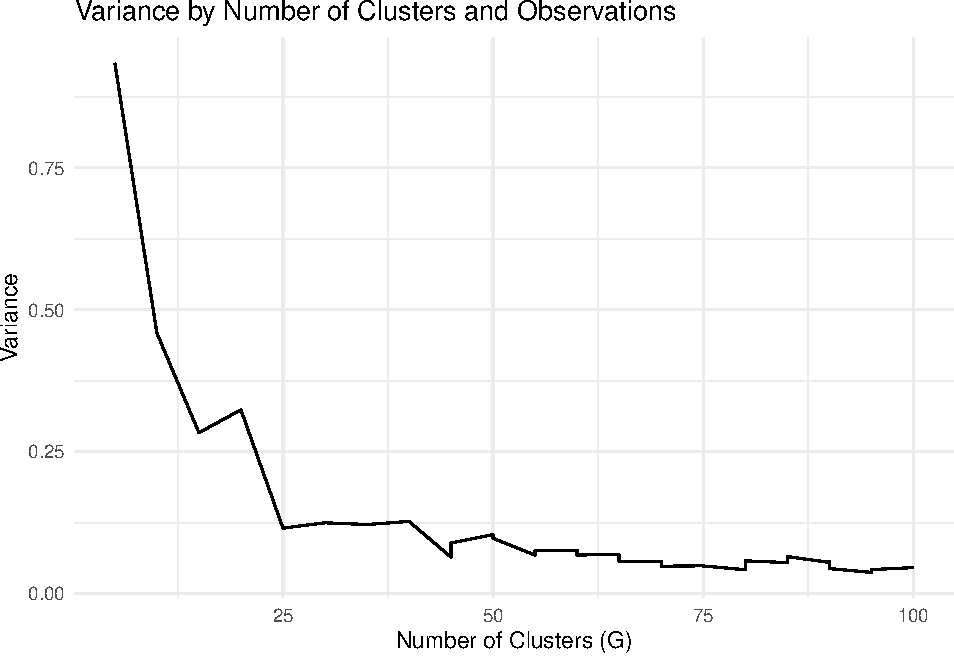
\includegraphics{Project3Simulation_files/figure-latex/unnamed-chunk-4-1} \end{center}

\hypertarget{optimal-design}{%
\section{Optimal Design}\label{optimal-design}}

The first plot illustrates the relationship between the number of
clusters (\(G\)) and the variance of the treatment effect estimate.
Variance decreases significantly as the number of clusters increases,
with a sharp decline up to around \(G = 25\), after which the reduction
becomes more gradual and stabilizes around \(G = 80\). This
stabilization suggests diminishing returns in variance reduction as
\(G\) increases. The optimal cluster size is identified as \(G = 80\),
marked with a red dashed line, where variance is sufficiently low,
balancing precision with the associated costs.

From the data table, the optimal configuration consists of \(G = 80\)
clusters, each with \(R = 19\) individuals per cluster. This
configuration yields a low variance of 0.035, a high cost efficiency of
0.0035, and an intraclass correlation coefficient (ICC) of 0.487,
indicating a balanced contribution of between-cluster variance to the
total variance. The total cost for this design is \$8000, which is well
within the specified budget constraint of \$10,000. This result
underscores the importance of optimizing \(G\) and \(R\) to achieve
precise estimates at a manageable cost.

\begin{verbatim}
##      G  R   variance beta alpha c1 c2 total_cost cost_efficiency       icc
## 200 80 19 0.03546992    1     0 10  5       8000     0.003524113 0.4879634
##         B gamma2 sigma2 precision
## 200 10000      1      1   28.1929
\end{verbatim}

\begin{center}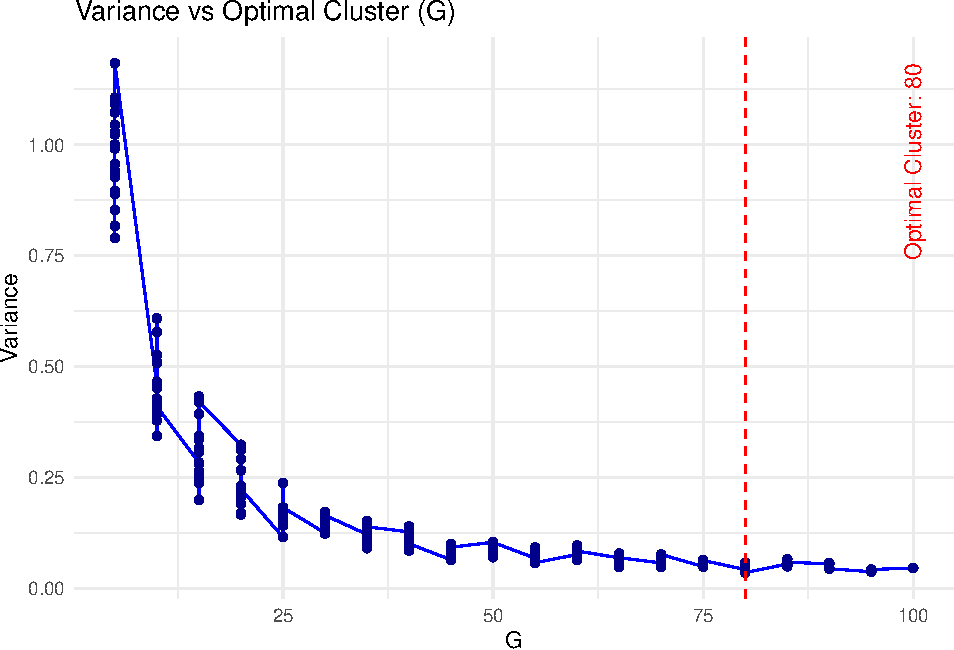
\includegraphics{Project3Simulation_files/figure-latex/unnamed-chunk-5-1} \end{center}

\hypertarget{correlation-within-clusters}{%
\section{Correlation within
Clusters}\label{correlation-within-clusters}}

The boxplot illustrates the distribution of the response variable Y
across five distinct clusters, revealing noticeable differences in
central tendency and variability. Cluster 3 has the lowest median,
indicating it tends to have lower responses, while Cluster 4 exhibits
the highest median, suggesting higher responses in that group.
Variability is greatest in Cluster 1, with a wide range and several
outliers, whereas Cluster 3 shows the least variability, with a more
concentrated distribution. Outliers are present in all clusters except
Cluster 4, indicating some extreme values that deviate from the primary
distribution. Comparatively, Clusters 4 and 5 have relatively similar
IQRs and higher medians, but Cluster 4's distribution is slightly
shifted upward.

\begin{center}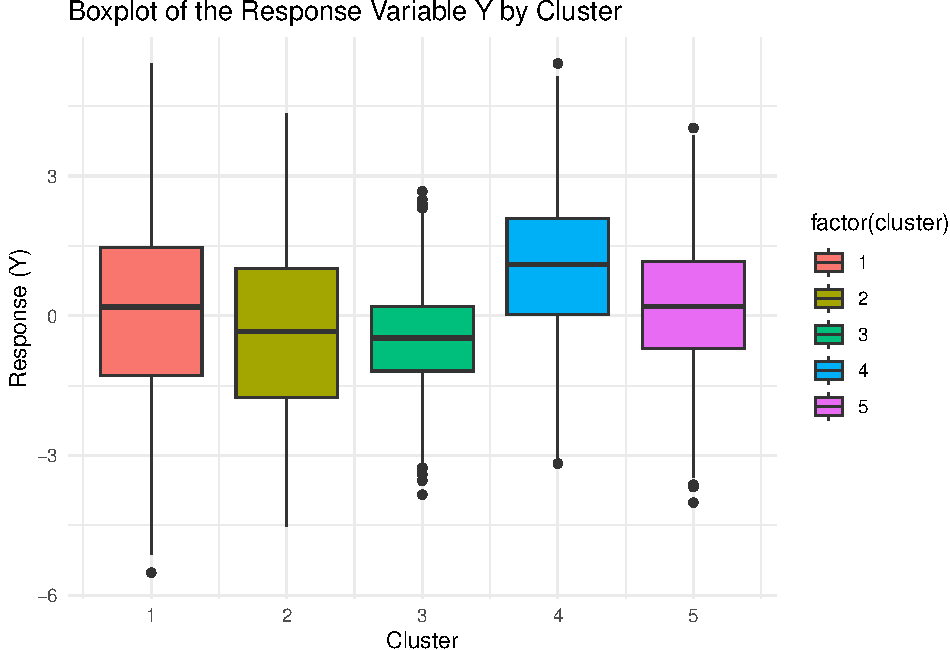
\includegraphics{Project3Simulation_files/figure-latex/unnamed-chunk-6-1} \end{center}

This boxplot illustrates the distribution of the response variable Y
across five clusters, stratified by treatment group (0 and 1), providing
insights into the relationship between clusters and treatment effects.
The variation in median values and spread within each cluster suggests
potential differences in how clusters are correlated with the response
variable. For Cluster 1, the treatment group (1) shows a higher median
and greater variability compared to the control group (0), indicating a
possible treatment effect within this cluster. Cluster 2 exhibits a
narrower gap between the groups, with similar variability, suggesting
weaker differentiation between treatment and control groups. In Cluster
3, the medians overlap substantially, implying minimal correlation
between treatment and response. Clusters 4 and 5 display more distinct
separation between treatment and control groups, with treatment group
medians consistently higher, suggesting a stronger treatment effect in
these clusters. These patterns highlight that treatment effects may vary
significantly by cluster, indicating that cluster membership is
correlated with the response and may influence the efficacy of the
treatment.

\begin{center}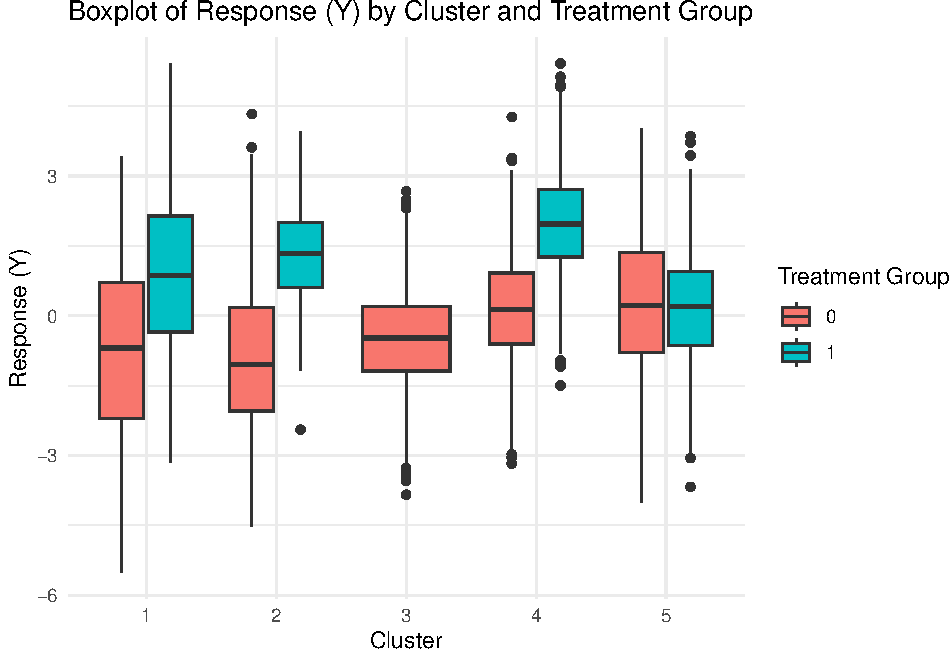
\includegraphics{Project3Simulation_files/figure-latex/unnamed-chunk-7-1} \end{center}

\hypertarget{highest-icc}{%
\section{Highest ICC}\label{highest-icc}}

The results indicate that with \(G = 5\) clusters and \(R = 32\)
individuals per cluster, the total variance of the outcome variable is
\(0.853\), and the intraclass correlation coefficient (ICC) is
\(0.749\). The high ICC suggests that approximately 74.9\% of the total
variance is due to between-cluster variability, with only about 25.1\%
arising from within-cluster differences. This highlights a strong
correlation among observations within the same cluster. The precision,
calculated as \(1/\text{variance}\), is \(1.172\), reflecting the
accuracy of the treatment effect estimate under this design. The total
cost of the design is \$825, demonstrating cost-efficiency
(\(0.00142\)), given the high ICC and the large proportion of
between-cluster variation.

In the context of this study, the high ICC underscores the importance of
accounting for clustering effects in the analysis to avoid
underestimating standard errors and overinflating the significance of
findings. It also suggests that increasing the number of clusters
(\(G\)) rather than adding more individuals per cluster (\(R\)) would be
a more effective strategy for improving precision, as additional
observations within a cluster contribute less unique information. This
design balances cost considerations with sufficient precision, making it
an appropriate choice for studies where between-cluster variability
dominates. These insights can guide future decisions on allocating
resources and optimizing study designs.

\begin{verbatim}
##   G  R  variance beta alpha c1 c2 total_cost cost_efficiency       icc     B
## 1 5 32 0.8533398    1     0 10  5        825     0.001420444 0.7497686 10000
##   gamma2 sigma2 precision
## 1      1      1  1.171866
\end{verbatim}

\begin{center}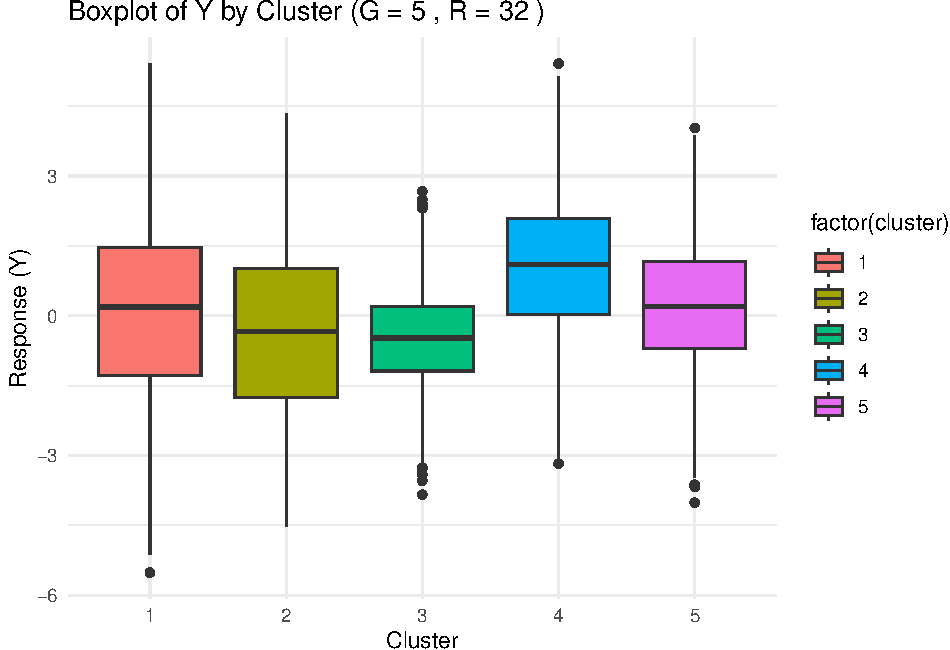
\includegraphics{Project3Simulation_files/figure-latex/unnamed-chunk-8-1} \end{center}

\hypertarget{least-icc}{%
\section{Least ICC}\label{least-icc}}

This boxplot shows the distribution of the response variable Y across
five clusters with the corresponding design parameters listed in the
table, characterized by the lowest intra-class correlation coefficient
(ICC = 0). The ICC of 0 indicates no correlation between observations
within the same cluster, implying that all variance in Y is attributed
to individual-level variation rather than group-level effects.

The distributions vary notably across clusters, with Cluster 1 showing
the highest median response and minimal spread, while Cluster 4 has a
notably lower median and larger variability. Clusters 2 and 3 have
relatively narrow ranges, suggesting limited dispersion in those groups.
Despite these differences, the ICC of 0 indicates that these patterns
are independent of within-cluster similarity, as no shared group-level
effects influence Y. This setup reflects an environment where clustering
may not significantly affect the response variable, focusing on
individual-level predictors.

The design parameters (G=5,R=20) and total cost (525) suggest that the
design is cost-efficient ( cost\_efficiency =0.0021), as resources are
allocated effectively to balance variance and group size. Overall, this
design is optimized for minimal group-level dependence, making it
suitable for scenarios where individual-level characteristics are
primary drivers of the response.

\begin{verbatim}
##   G  R  variance beta alpha c1 c2 total_cost cost_efficiency icc     B gamma2
## 1 5 20 0.8893293    1     0 10  5        525     0.002141796   0 10000      1
##   sigma2 precision
## 1      1  1.124443
\end{verbatim}

\begin{center}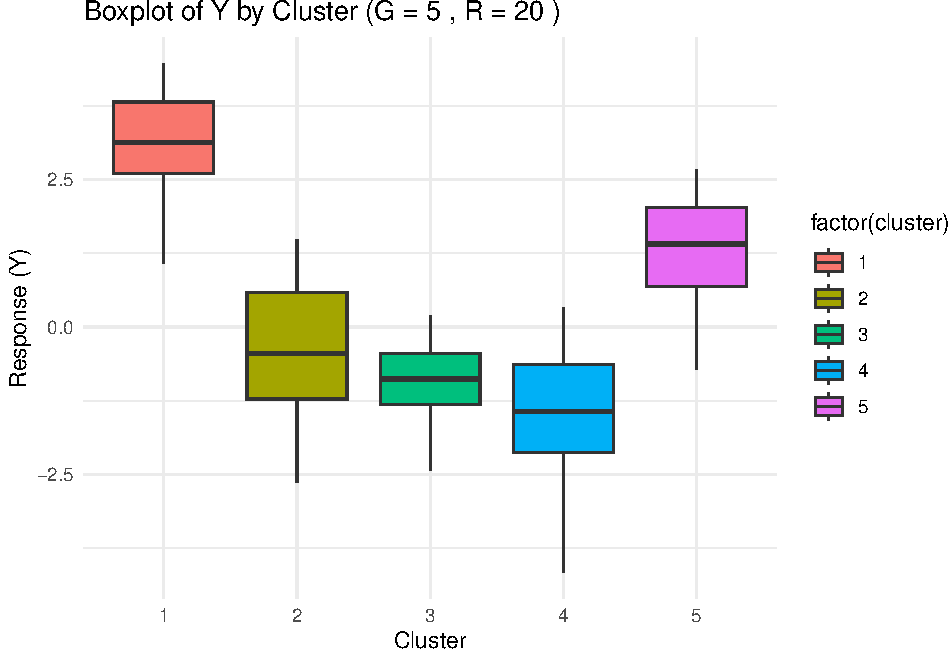
\includegraphics{Project3Simulation_files/figure-latex/unnamed-chunk-9-1} \end{center}

\hypertarget{varied-gamma-and-sigma}{%
\section{Varied Gamma and Sigma}\label{varied-gamma-and-sigma}}

\hypertarget{gamma-3-results}{%
\subsection{Gamma 3 Results}\label{gamma-3-results}}

This plot illustrates how cost efficiency varies with the number of
clusters (\(G\)) for a fixed \(\gamma = 0.5\), across different sample
sizes (\(R\)). Cost efficiency fluctuates significantly for smaller
sample sizes (\(R = 19, 20, 25\)), indicating sensitivity to changes in
the number of clusters when within-cluster resources are limited. As
\(R\) increases (e.g., \(R = 39, 43, 65\)), the variability in cost
efficiency reduces, suggesting more stable performance in resource
allocation across different cluster sizes. For the largest values of
\(R\) (e.g., \(R = 99, 132, 199\)), cost efficiency remains consistently
low, indicating optimal resource use with minimal sensitivity to cluster
count.

This plot demonstrates the impact of a fixed \(\sigma = 2\)
(individual-level random effects variance) on cost efficiency across
different numbers of clusters (\(G\)) and sample sizes per cluster
(\(R\)). Cost efficiency fluctuates more for smaller \(R\) values (
\(R = 19, 20, 25\)), reflecting sensitivity to cluster configurations
when individual-level variability is prominent. As \(R\) increases, the
fluctuations in cost efficiency stabilize, with larger \(R\) values (
\(R = 79, 99, 132\)) showing consistently low cost efficiency values,
indicating optimal resource utilization with minimal variability across
different cluster counts.

\hypertarget{sigma-3-results}{%
\subsection{Sigma 3 Results}\label{sigma-3-results}}

\begin{center}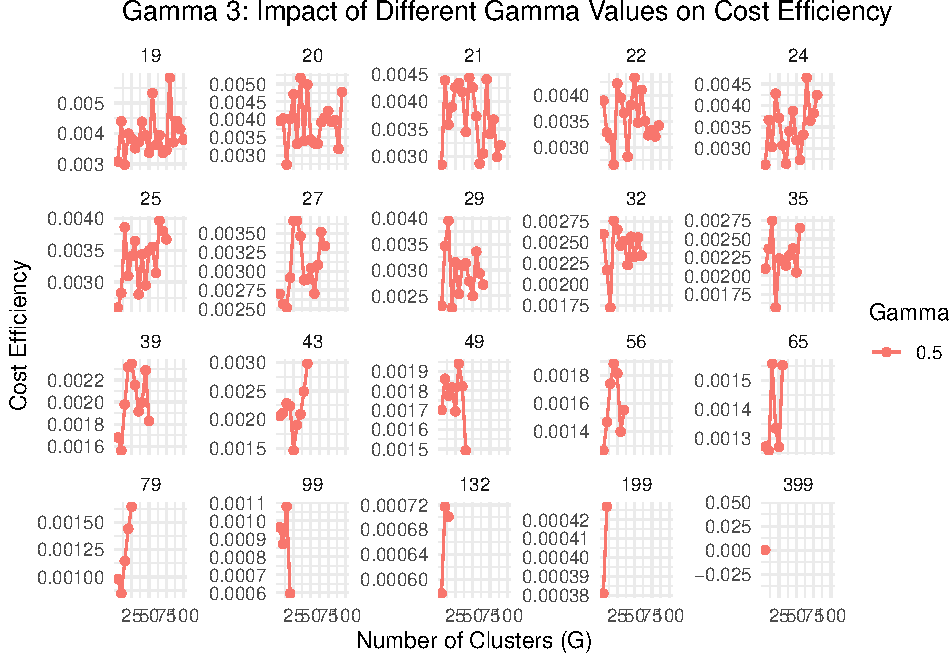
\includegraphics{Project3Simulation_files/figure-latex/unnamed-chunk-10-1} \end{center}

\begin{center}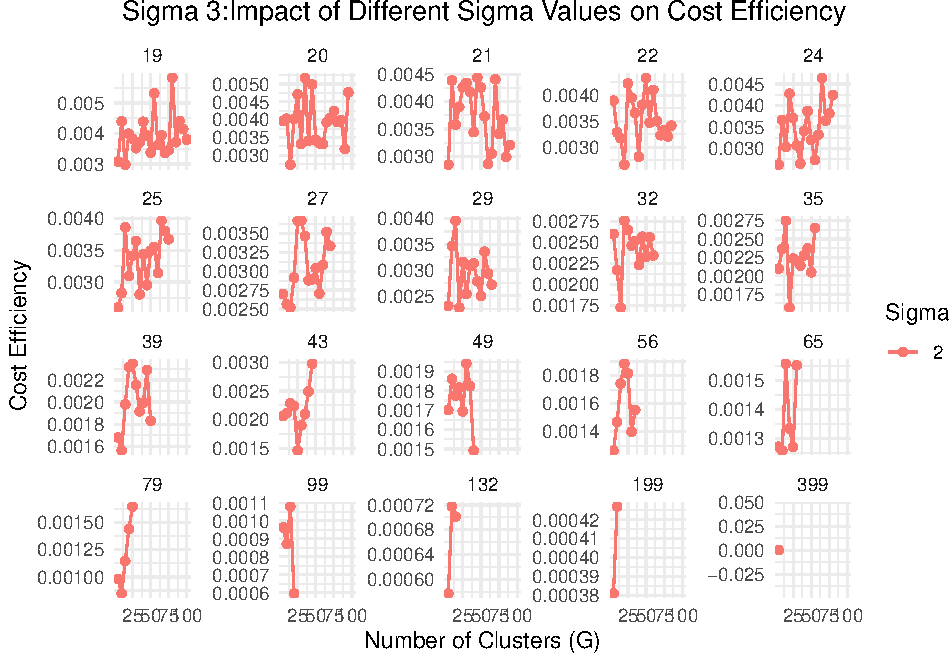
\includegraphics{Project3Simulation_files/figure-latex/unnamed-chunk-10-2} \end{center}

\hypertarget{optimal-results-3}{%
\subsection{Optimal Results 3}\label{optimal-results-3}}

These results present the optimal the cluster which is 95.

\begin{verbatim}
##      G  R   variance beta alpha c1 c2 total_cost cost_efficiency       icc
## 208 95 20 0.02103523    1     0 10  5       9975     0.004765844 0.1863396
##         B gamma2 sigma2 precision
## 208 10000    0.5      2   47.5393
\end{verbatim}

\begin{center}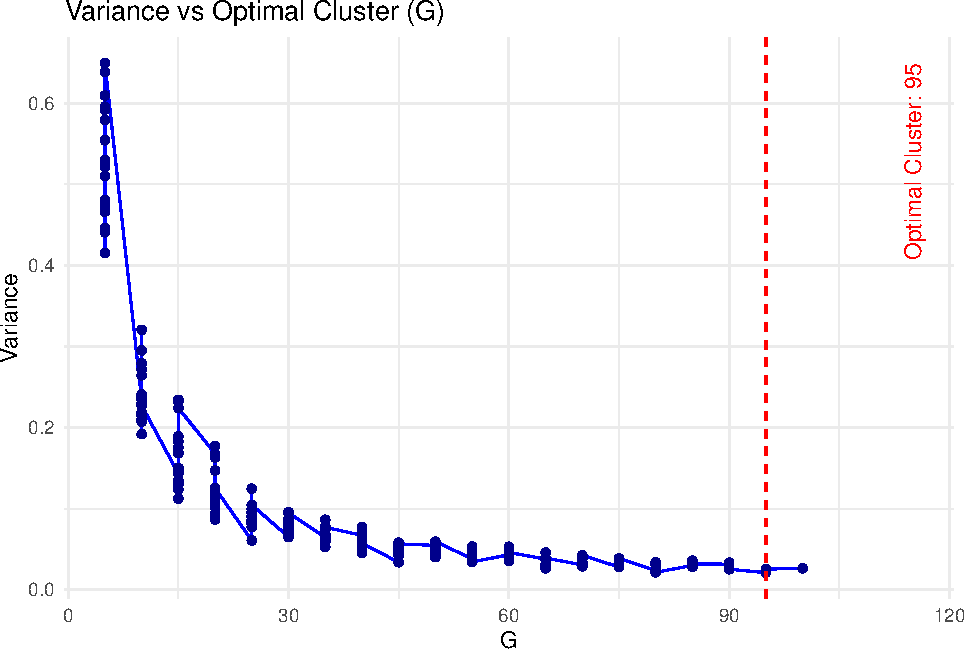
\includegraphics{Project3Simulation_files/figure-latex/unnamed-chunk-11-1} \end{center}

\hypertarget{gamma-4-results}{%
\section{Gamma 4 Results}\label{gamma-4-results}}

This plot illustrates the effect of \(\gamma = 2\) (variance of
cluster-level random effects) on cost efficiency across varying cluster
sizes (\(G\)) and sample sizes (\(R\)). For smaller \(R\) values (e.g.,
\(R = 19, 20, 25\)), cost efficiency fluctuates significantly,
indicating high sensitivity to changes in cluster size when
cluster-level variance is substantial. As \(R\) increases (e.g.,
\(R = 79, 99, 132\)), cost efficiency stabilizes at consistently low
values, suggesting optimal resource allocation with reduced sensitivity
to the number of clusters when within-cluster sample sizes are
sufficient.

\hypertarget{sigma-4-results}{%
\section{Sigma 4 Results}\label{sigma-4-results}}

This plot explores the impact of \(\sigma = 3\) (individual-level random
effects variance) on cost efficiency across varying cluster sizes
(\(G\)) and sample sizes (\(R\)). For smaller \(R\) values (e.g.,
\(R = 19, 20, 25\)), cost efficiency fluctuates significantly,
indicating sensitivity to changes in \(G\), as higher individual-level
variance increases the need for precise resource allocation. As \(R\)
increases, the variability in cost efficiency stabilizes, with
consistently lower values for larger \(R\) (e.g., \(R = 79, 99, 132\)),
reflecting optimal resource utilization and reduced sensitivity to
cluster count when within-cluster sample sizes are sufficient. This
pattern highlights that higher individual-level variance amplifies the
influence of smaller sample sizes on cost efficiency, requiring careful
balancing of cluster and sample size configurations.

\begin{center}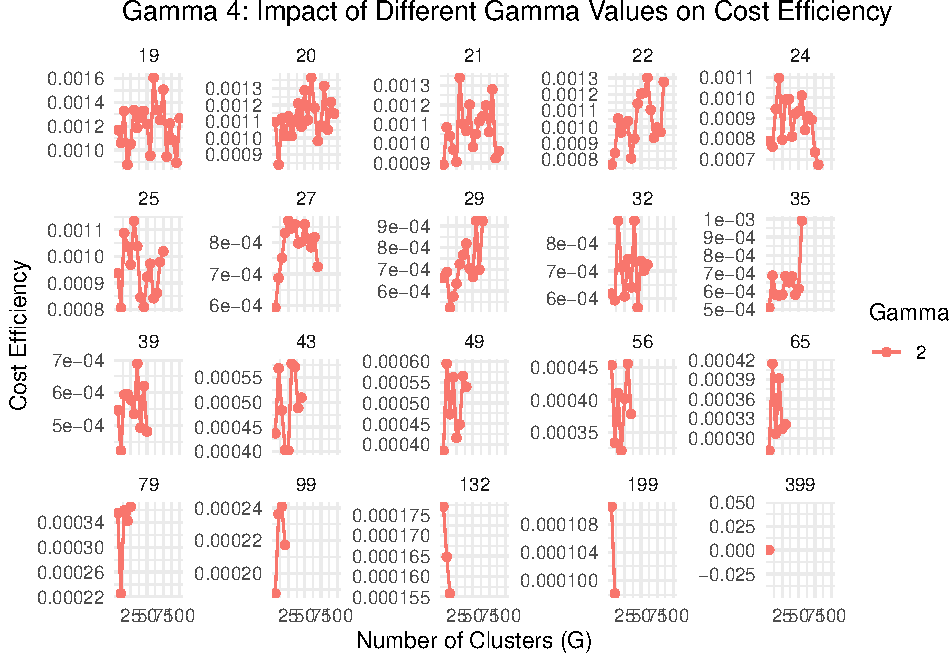
\includegraphics{Project3Simulation_files/figure-latex/unnamed-chunk-12-1} \end{center}

\begin{center}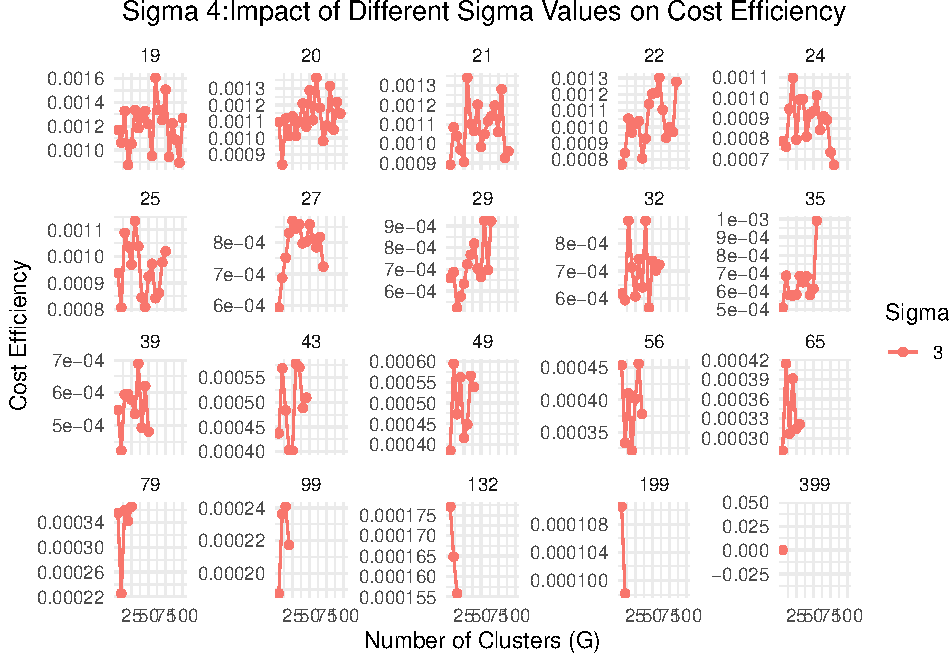
\includegraphics{Project3Simulation_files/figure-latex/unnamed-chunk-12-2} \end{center}

\#Optimal Results The optimal cluster is 80.

\begin{verbatim}
##       G  R   variance beta alpha c1 c2 total_cost cost_efficiency       icc
## 210 100 19 0.07894768    1     0 10  5      10000     0.001266662 0.4105546
##         B gamma2 sigma2 precision
## 210 10000      2      3  12.66662
\end{verbatim}

\begin{center}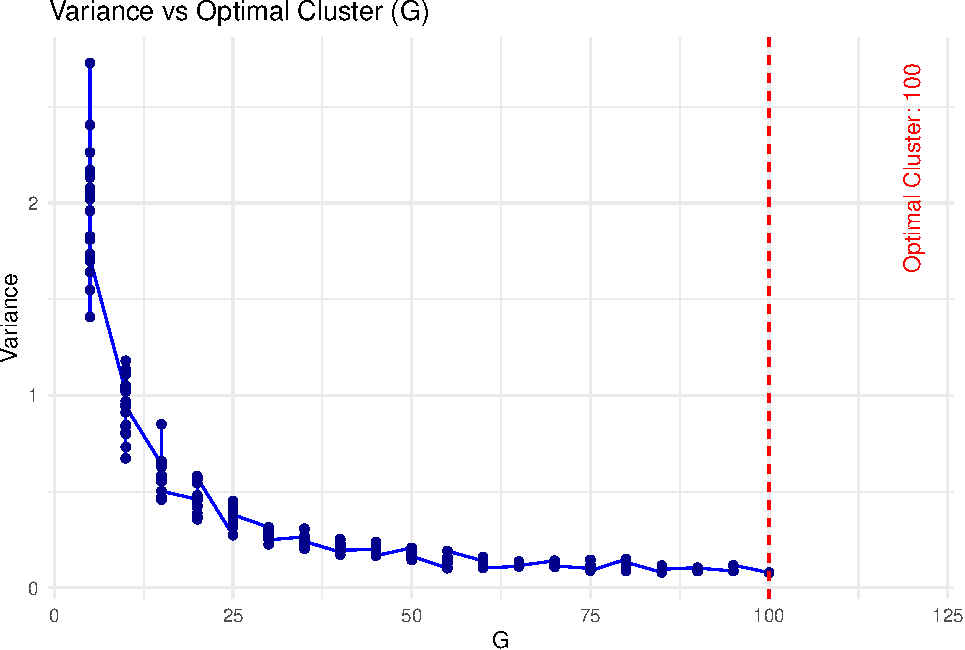
\includegraphics{Project3Simulation_files/figure-latex/unnamed-chunk-13-1} \end{center}

\hypertarget{gamma-5-results}{%
\section{Gamma 5 Results}\label{gamma-5-results}}

This plot shows the impact of \(\gamma = 3\) (cluster-level random
effects variance) on cost efficiency across different cluster sizes
(\(G\)) and sample sizes (\(R\)). For smaller \(R\) values (e.g.,
\(R = 19, 20, 25\)), cost efficiency exhibits substantial variability,
reflecting high sensitivity to changes in \(G\) due to increased
cluster-level variance. As \(R\) increases (e.g., \(R = 79, 99, 132\)),
cost efficiency stabilizes at consistently lower values, indicating that
larger sample sizes mitigate the effects of high cluster-level variance,
leading to more efficient designs. These results highlight the
importance of balancing \(G\) and \(R\) to optimize cost efficiency
under significant cluster-level variability.

\hypertarget{sigma-5-results}{%
\section{Sigma 5 Results}\label{sigma-5-results}}

This plot highlights the impact of \(\sigma = 4\) (individual-level
random effects variance) on cost efficiency across varying cluster sizes
(\(G\)) and sample sizes (\(R\)). For smaller \(R\) values (e.g.,
\(R = 19, 20, 25\)), cost efficiency fluctuates significantly,
reflecting sensitivity to both \(\sigma\) and cluster configuration,
with high variability reducing resource optimization. As \(R\) increases
(e.g., \(R = 79, 99, 132\)), cost efficiency stabilizes at lower values,
indicating improved efficiency and reduced sensitivity to \(\sigma\) as
sample sizes grow. These results emphasize that larger individual-level
variance amplifies inefficiencies at smaller sample sizes, making larger
within-cluster sample sizes critical for achieving optimal designs.

\begin{center}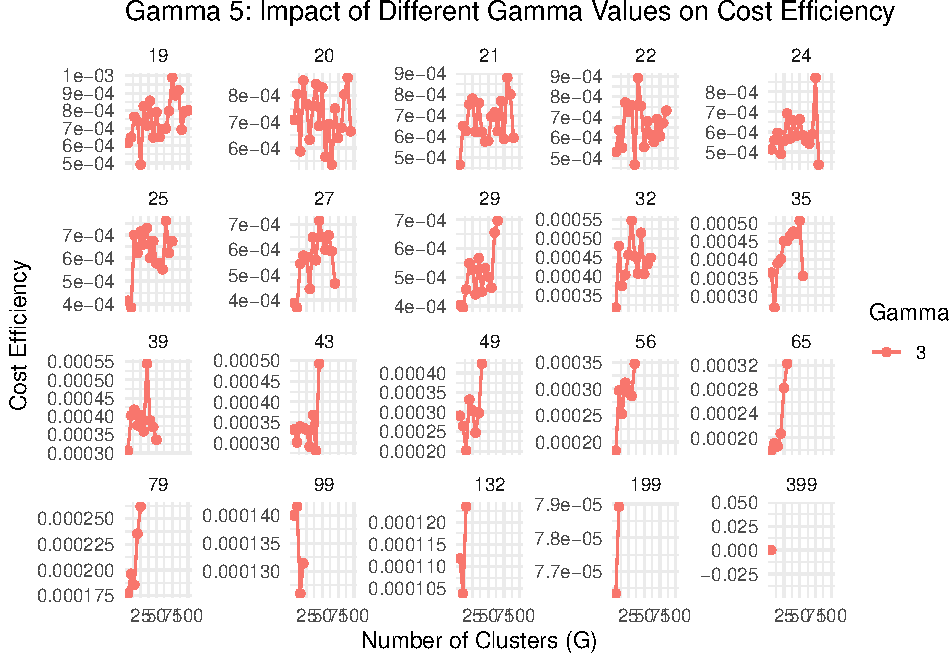
\includegraphics{Project3Simulation_files/figure-latex/unnamed-chunk-14-1} \end{center}

\begin{center}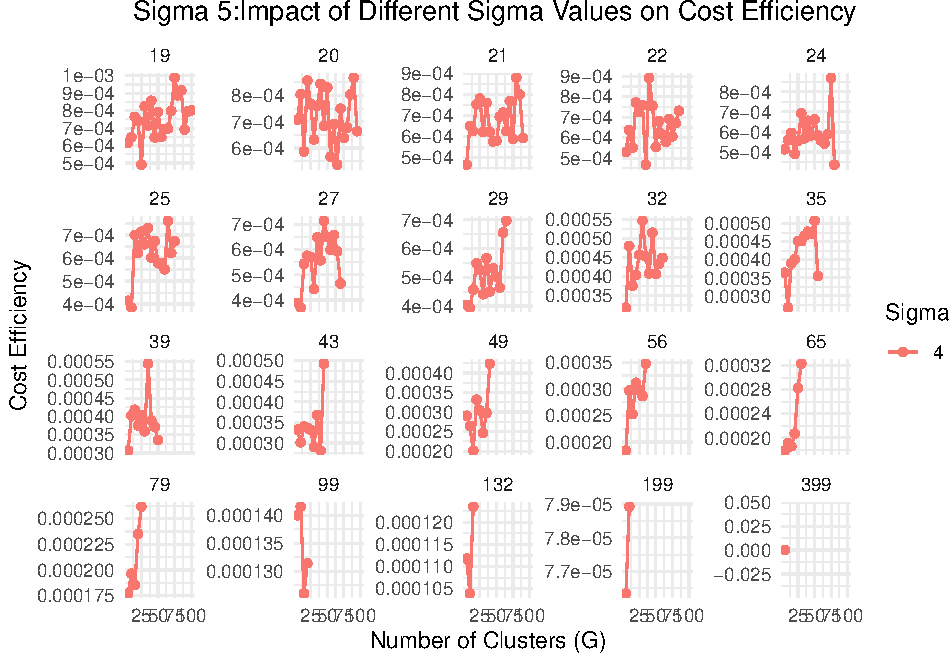
\includegraphics{Project3Simulation_files/figure-latex/unnamed-chunk-14-2} \end{center}

\#\#Optimal Results 5

The optimal cluster is 90.

\begin{verbatim}
##      G  R  variance beta alpha c1 c2 total_cost cost_efficiency       icc     B
## 206 90 20 0.1219878    1     0 10  5       9450    0.0008674644 0.4333895 10000
##     gamma2 sigma2 precision
## 206      3      4  8.197539
\end{verbatim}

\begin{center}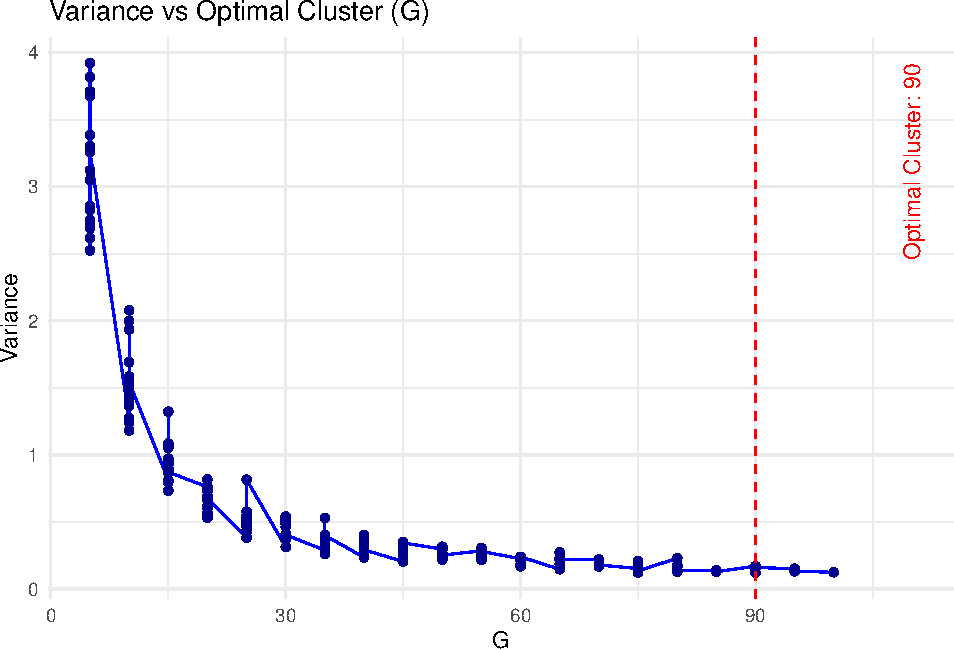
\includegraphics{Project3Simulation_files/figure-latex/unnamed-chunk-15-1} \end{center}

\hypertarget{overall-varoid-gamma-and-sigma}{%
\subsection{Overall Varoid Gamma and
Sigma}\label{overall-varoid-gamma-and-sigma}}

The variations in \(\gamma\) (cluster-level random effects variance)
significantly impact cost efficiency by altering the sensitivity of the
results to the number of clusters (\(G\)) and sample sizes per cluster
(\(R\)). Higher \(\gamma\) values (e.g., \(\gamma = 3\)) increase
sensitivity to \(G\), particularly at smaller \(R\), as greater
between-cluster variability necessitates precise tuning of cluster
numbers to optimize resource allocation. Conversely, lower \(\gamma\)
values (e.g., \(\gamma = 0.5\)) produce more stable cost efficiency
across varying \(G\), making the design less sensitive to cluster
configurations. At higher \(R\), cost efficiency stabilizes for all
\(\gamma\) values, though larger \(\gamma\) requires greater
within-cluster sample sizes to achieve similar levels of efficiency.
Overall, higher \(\gamma\) amplifies inefficiencies in smaller sample
designs, emphasizing the need for careful balancing of \(G\) and \(R\)
to account for increased cluster-level variability and ensure
cost-effective study designs.

The variations in \(\sigma\) (individual-level random effects variance)
significantly influence cost efficiency by affecting the sensitivity of
results to the number of clusters (\(G\)) and sample sizes per cluster
(\(R\)). Higher \(\sigma\) values (e.g., \(\sigma = 4\)) amplify
variability within clusters, leading to greater fluctuations in cost
efficiency at smaller \(R\), as higher individual-level noise requires
larger sample sizes to maintain precision. In contrast, lower \(\sigma\)
values (e.g., \(\sigma = 2\)) result in more stable cost efficiency
across cluster configurations, reducing the sensitivity to changes in
\(G\). At higher \(R\), cost efficiency stabilizes for all \(\sigma\)
values, though higher \(\sigma\) necessitates larger within-cluster
sample sizes to counteract the increased variability and achieve optimal
efficiency. Overall, larger \(\sigma\) values magnify inefficiencies in
smaller sample designs, highlighting the importance of adequately
increasing \(R\) to mitigate individual-level noise and ensure effective
resource allocation.

\hypertarget{varied-costs-c1-and-c2}{%
\section{Varied costs (c1 and c2)}\label{varied-costs-c1-and-c2}}

In my Results 6 Evaluation, the c1 cost was adjusted to 30 dollars and
the c2 was kept the same at 5 dollars. In my Results 7 Evaluation, the
c1 cost was adjusted to 30 dollars and c2 was adjusted to 2 dollars.In
my Results 8 Evaluation, the c1 cost was adjusted to 50 dollars and the
c2 was kept the same at 5 dollars. In my Results 9 Evaluation, the c1
cost was adjusted to 50 dollars and the c2 was adjusted to \$10. Going
through through the evaluation design, I noticed how the G and R
adjusted, causing less observations in R.The cost also increased as the
the c1 and c2 shifted as well.

\begin{verbatim}
##      G  R   variance beta alpha c1 c2 total_cost cost_efficiency       icc
## 200 80 19 0.03546992    1     0 10  5       8000     0.003524113 0.4879634
##         B gamma2 sigma2 precision
## 200 10000      1      1   28.1929
\end{verbatim}

\begin{center}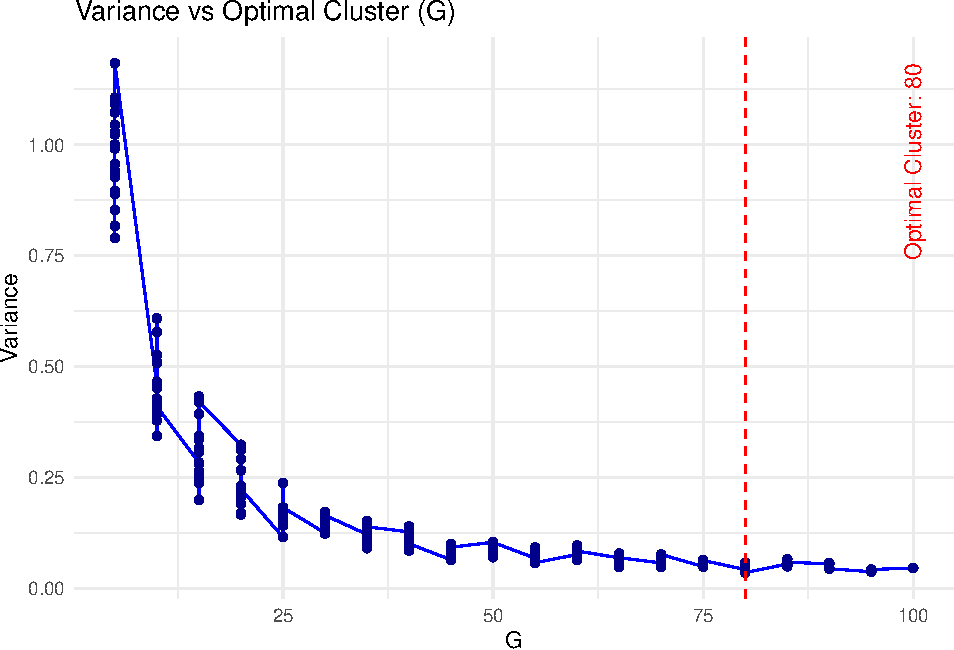
\includegraphics{Project3Simulation_files/figure-latex/unnamed-chunk-16-1} \end{center}

This visualization examines the relationship between cost efficiency and
the number of clusters (\(G\)) across different sample sizes per cluster
(\(R\)). The results reveal that cost efficiency fluctuates moderately
as \(G\) increases for smaller \(R\) values ( \(R = 19, 20, 25\)), with
notable peaks and troughs suggesting sensitivity to cluster size when
sample sizes are limited. As \(R\) increases (\(R = 43, 49, 56, 65\)),
the cost efficiency trends become more stable, indicating that larger
sample sizes mitigate the impact of changes in \(G\).

For intermediate \(R\) values (e.g., \(R = 25, 29\)), cost efficiency
often reaches optimal levels at moderate \(G\) values, reflecting a
balance between distributing resources across clusters and maintaining
sufficient within-cluster observations. At very high \(R\) values (e.g.,
\(R = 99, 132, 199\)), cost efficiency is consistently low, with minimal
fluctuation regardless of \(G\), indicating that high within-cluster
sample sizes reduce the sensitivity to cluster count.

Overall, the findings suggest that the relationship between \(G\) and
cost efficiency is influenced by the sample size per cluster, with
smaller \(R\) requiring careful tuning of \(G\) to optimize efficiency,
while higher \(R\) stabilizes performance across a wider range of
cluster configurations. This highlights the importance of balancing
\(G\) and \(R\) to achieve cost-effective designs within the constraints
of a study.

\begin{center}\includegraphics{Project3Simulation_files/figure-latex/unnamed-chunk-20-1} \end{center}

\hypertarget{results-7-plot}{%
\section{Results 7 Plot}\label{results-7-plot}}

This visualization explores the relationship between cost efficiency and
the number of clusters (\(G\)) across varying sample sizes per cluster
(\(R\)). The results indicate that cost efficiency exhibits moderate
fluctuations as \(G\) increases for smaller sample sizes
(\(R = 19, 20, 21\)), with noticeable peaks , suggesting that optimal
cluster configurations are more sensitive when fewer observations per
cluster are available. As \(R\) increases (\(R = 25, 27, 29\)), the
fluctuations in cost efficiency smooth out, indicating improved
stability in the allocation of resources across cluster configurations.

At higher values of \(R\) ( \(R = 43, 49, 56, 65\)), cost efficiency
stabilizes further, with minimal sensitivity to changes in \(G\). This
trend suggests that larger within-cluster sample sizes mitigate the
effect of increasing cluster numbers, likely due to sufficient
representation within each group. For the highest \(R\) values (e.g.,
\(R = 79, 99, 132\)), cost efficiency remains consistently low across
all \(G\), reflecting optimal resource utilization and reduced
dependency on cluster count.

Overall, the findings highlight that the interplay between \(G\) and
\(R\) is a critical factor in optimizing cost efficiency. Smaller \(R\)
values necessitate careful tuning of \(G\) to achieve efficiency, while
larger \(R\) values reduce the need for precise adjustments, offering
more flexibility in cluster design. These insights are crucial for
designing cost-effective studies that balance cluster count and sample
size within resource constraints.

\begin{center}\includegraphics{Project3Simulation_files/figure-latex/unnamed-chunk-21-1} \end{center}

\hypertarget{results-8-plot}{%
\subsection{Results 8 Plot}\label{results-8-plot}}

This visualization illustrates the relationship between cost efficiency
and the number of clusters (\(G\)), faceted by different sample sizes
per cluster (\(R\)). Across most values of \(R\), cost efficiency
fluctuates with changes in \(G\), though the magnitude and patterns of
fluctuation vary. For smaller \(R\) values (e.g., \(R = 19, 20, 25\)),
there is more pronounced variability in cost efficiency as \(G\)
increases, suggesting that optimizing cluster size plays a more critical
role in resource allocation when per-cluster sample sizes are smaller.
At higher \(R\) values (e.g., \(R = 43, 49, 65\)), the cost efficiency
stabilizes, with smaller deviations as \(G\) increases, indicating
diminishing returns in adjusting \(G\) when sample sizes are
sufficiently large.

Notably, for intermediate \(R\) values such as \(R = 25\) or \(R = 29\),
peaks in cost efficiency occur at moderate \(G\) values, highlighting an
optimal balance where resources are neither too dispersed across too
many clusters nor concentrated in too few. For very large \(R\) values
(e.g., \(R = 99, 132, 199\)), cost efficiency remains nearly constant
regardless of \(G\), reflecting that higher sample sizes per cluster
mitigate the effect of cluster count on resource allocation.

Overall, the results indicate that the interplay between \(G\) and \(R\)
significantly influences cost efficiency, with the optimal number of
clusters depending on the sample size per cluster and the budget
constraints. These findings emphasize the importance of tailoring \(G\)
and \(R\) to the study design goals and available resources.

\begin{center}\includegraphics{Project3Simulation_files/figure-latex/unnamed-chunk-22-1} \end{center}

\hypertarget{results-plot-9}{%
\subsection{Results Plot 9}\label{results-plot-9}}

This visualization illustrates the relationship between cost efficiency
and the number of clusters (\(G\)), faceted by the sample size per
cluster (\(R\)). The cost efficiency tends to fluctuate as \(G\)
increases, with varying trends across different values of \(R\). For
smaller values of \(R\), such as 19 or 20, cost efficiency exhibits
relatively minor variability across the range of \(G\), indicating
consistent allocation of resources. However, as \(R\) increases (e.g.,
\(R = 43, 56, 65\)), the patterns become more irregular, suggesting that
higher \(R\) introduces greater sensitivity to changes in \(G\).

Notably, cost efficiency is generally lower (closer to optimal) for
moderate values of \(G\), with some dips observed in certain scenarios,
reflecting improved resource utilization. Extreme values of \(G\),
either very small or very large, often result in higher (less efficient)
cost efficiency values. This pattern underscores the trade-off between
dividing resources across many clusters (large \(G\)) and ensuring
sufficient sample sizes within each cluster (larger \(R\)). The results
suggest that optimal cost efficiency is achieved at a balance point
where \(G\) and \(R\) are neither too small nor too large, and this
balance depends on the overall study design and resource allocation
constraints.

\begin{center}\includegraphics{Project3Simulation_files/figure-latex/unnamed-chunk-23-1} \end{center}

\hypertarget{aim-3-poisson-regression-model}{%
\section{Aim 3 : Poisson Regression
Model}\label{aim-3-poisson-regression-model}}

\hypertarget{poisson-distribution}{%
\subsection{Poisson Distribution}\label{poisson-distribution}}

\hypertarget{section}{%
\section{}\label{section}}

\hypertarget{section-1}{%
\section{}\label{section-1}}

\hypertarget{section-2}{%
\section{}\label{section-2}}

\hypertarget{set.seed222}{%
\section{set.seed(222)}\label{set.seed222}}

\hypertarget{section-3}{%
\section{}\label{section-3}}

\hypertarget{function-to-simulate-data}{%
\section{\# Function to simulate data}\label{function-to-simulate-data}}

\hypertarget{data_simulated---functiong-r-alpha-beta-gamma2-sigma2-treatment_prob-0.5}{%
\section{data\_simulated \textless- function(G, R, alpha, beta, gamma2,
sigma2, treatment\_prob = 0.5)
\{}\label{data_simulated---functiong-r-alpha-beta-gamma2-sigma2-treatment_prob-0.5}}

\hypertarget{generate-cluster-level-treatment-assignment}{%
\section{\# Generate cluster-level treatment
assignment}\label{generate-cluster-level-treatment-assignment}}

\hypertarget{x---rbinomg-1-treatment_prob-randomly-assign-treatment-1-or-control-0-to-clusters}{%
\section{X \textless- rbinom(G, 1, treatment\_prob) \# Randomly assign
treatment (1) or control (0) to
clusters}\label{x---rbinomg-1-treatment_prob-randomly-assign-treatment-1-or-control-0-to-clusters}}

\hypertarget{section-4}{%
\section{}\label{section-4}}

\hypertarget{generate-cluster-level-random-effects}{%
\section{\# Generate cluster-level random
effects}\label{generate-cluster-level-random-effects}}

\hypertarget{epsilon---rnormg-mean-0-sd-sqrtgamma2}{%
\section{epsilon \textless- rnorm(G, mean = 0, sd =
sqrt(gamma2))}\label{epsilon---rnormg-mean-0-sd-sqrtgamma2}}

\hypertarget{section-5}{%
\section{}\label{section-5}}

\hypertarget{generate-individual-level-observations}{%
\section{\# Generate individual-level
observations}\label{generate-individual-level-observations}}

\hypertarget{data---data.frame}{%
\section{data \textless- data.frame(}\label{data---data.frame}}

\hypertarget{cluster-rep1g-each-r}{%
\section{cluster = rep(1:G, each = R),}\label{cluster-rep1g-each-r}}

\hypertarget{x-repx-each-r}{%
\section{X = rep(X, each = R)}\label{x-repx-each-r}}

\hypertarget{section-6}{%
\section{)}\label{section-6}}

\hypertarget{section-7}{%
\section{}\label{section-7}}

\hypertarget{epsilon---repepsilon-each-r-repeat-cluster-level-random-effects-for-all-individuals-in-the-cluster}{%
\section{epsilon \textless- rep(epsilon, each = R) \# Repeat
cluster-level random effects for all individuals in the
cluster}\label{epsilon---repepsilon-each-r-repeat-cluster-level-random-effects-for-all-individuals-in-the-cluster}}

\hypertarget{mu---expalpha-beta-datax-epsilon-datay---rpoisn-nrowdata-lambda-mu}{%
\section{\texorpdfstring{Mu \textless- exp(alpha + beta *
data\(X + epsilon) # data\)Y \textless- rpois(n = nrow(data), lambda =
Mu)}{Mu \textless- exp(alpha + beta * dataX + epsilon) \# dataY \textless- rpois(n = nrow(data), lambda = Mu)}}\label{mu---expalpha-beta-datax-epsilon-datay---rpoisn-nrowdata-lambda-mu}}

\hypertarget{section-8}{%
\section{}\label{section-8}}

\hypertarget{returndata}{%
\section{return(data)}\label{returndata}}

\hypertarget{section-9}{%
\section{\}}\label{section-9}}

\hypertarget{section-10}{%
\section{}\label{section-10}}

\hypertarget{function-to-evaluate-designs}{%
\section{\# Function to evaluate
designs}\label{function-to-evaluate-designs}}

\hypertarget{evaluate_design2---functiong-r-alpha-beta-gamma2-c1-c2-b-n_sim}{%
\section{evaluate\_design2 \textless- function(G, R, alpha, beta,
gamma2, c1, c2, B, n\_sim)
\{}\label{evaluate_design2---functiong-r-alpha-beta-gamma2-c1-c2-b-n_sim}}

\hypertarget{results---data.frame}{%
\section{results \textless- data.frame(}\label{results---data.frame}}

\hypertarget{g-integer}{%
\section{G = integer(),}\label{g-integer}}

\hypertarget{r-integer}{%
\section{R = integer(),}\label{r-integer}}

\hypertarget{bias-numeric}{%
\section{bias = numeric(),}\label{bias-numeric}}

\hypertarget{variance-numeric}{%
\section{variance = numeric(),}\label{variance-numeric}}

\hypertarget{munumeric}{%
\section{Mu=numeric(),}\label{munumeric}}

\hypertarget{total_cost-numeric}{%
\section{total\_cost = numeric(),}\label{total_cost-numeric}}

\hypertarget{cost_efficiency-numeric}{%
\section{cost\_efficiency = numeric()}\label{cost_efficiency-numeric}}

\hypertarget{section-11}{%
\section{)}\label{section-11}}

\hypertarget{section-12}{%
\section{}\label{section-12}}

\hypertarget{for-g-in-g}{%
\section{for (g in G) \{}\label{for-g-in-g}}

\hypertarget{for-r-in-r}{%
\section{for (r in R) \{}\label{for-r-in-r}}

\hypertarget{check-budget-constraint}{%
\section{\# Check budget constraint}\label{check-budget-constraint}}

\hypertarget{total_cost---g-c1-g-r---1-c2}{%
\section{total\_cost \textless- g * c1 + g * (r - 1) *
c2}\label{total_cost---g-c1-g-r---1-c2}}

\hypertarget{if-total_cost-b-next-skip-if-over-budget}{%
\section{if (total\_cost \textgreater{} B) next \# Skip if over
budget}\label{if-total_cost-b-next-skip-if-over-budget}}

\hypertarget{section-13}{%
\section{}\label{section-13}}

\hypertarget{beta_estimates---numericn_sim}{%
\section{beta\_estimates \textless-
numeric(n\_sim)}\label{beta_estimates---numericn_sim}}

\hypertarget{section-14}{%
\section{}\label{section-14}}

\hypertarget{for-sim-in-1n_sim}{%
\section{for (sim in 1:n\_sim) \{}\label{for-sim-in-1n_sim}}

\hypertarget{data2---data_simulatedg-g-r-r-alpha-alpha-beta-beta-gamma2-gamma2-sigma2-0}{%
\section{data2 \textless- data\_simulated(G = g, R = r, alpha = alpha,
beta = beta, gamma2 = gamma2, sigma2 =
0)}\label{data2---data_simulatedg-g-r-r-alpha-alpha-beta-beta-gamma2-gamma2-sigma2-0}}

\hypertarget{section-15}{%
\section{}\label{section-15}}

\hypertarget{fit-poisson-mixed-effects-model}{%
\section{\# Fit Poisson mixed-effects
model}\label{fit-poisson-mixed-effects-model}}

\hypertarget{model---glmery-x-1-cluster-data-data2-family-poisson}{%
\section{model \textless- glmer(Y \textasciitilde{} X + (1 \textbar{}
cluster), data = data2, family =
poisson)}\label{model---glmery-x-1-cluster-data-data2-family-poisson}}

\hypertarget{beta_estimatessim---fixefmodelx-extract-estimate-for-beta}{%
\section{beta\_estimates{[}sim{]} \textless- fixef(model){[}``X''{]} \#
Extract estimate for
beta}\label{beta_estimatessim---fixefmodelx-extract-estimate-for-beta}}

\hypertarget{section-16}{%
\section{\}}\label{section-16}}

\hypertarget{section-17}{%
\section{}\label{section-17}}

\hypertarget{section-18}{%
\section{}\label{section-18}}

\hypertarget{section-19}{%
\section{}\label{section-19}}

\hypertarget{calculate-performance-metrics}{%
\section{\# Calculate performance
metrics}\label{calculate-performance-metrics}}

\hypertarget{section-20}{%
\section{}\label{section-20}}

\hypertarget{variance---varbeta_estimatesna.rmt}{%
\section{variance \textless-
var(beta\_estimates,na.rm=T)}\label{variance---varbeta_estimatesna.rmt}}

\hypertarget{random_effects_variance---as.numericvarcorrmodelcluster1-gamma2}{%
\section{random\_effects\_variance \textless-
as.numeric(VarCorr(model)\$cluster{[}1{]}) \#
gamma\^{}2}\label{random_effects_variance---as.numericvarcorrmodelcluster1-gamma2}}

\hypertarget{residual_variance---attrvarcorrmodel-sc2-sigma2}{%
\section{residual\_variance \textless- attr(VarCorr(model), ``sc'')\^{}2
\# sigma\^{}2}\label{residual_variance---attrvarcorrmodel-sc2-sigma2}}

\hypertarget{section-21}{%
\section{}\label{section-21}}

\hypertarget{calculate-icc}{%
\section{\# Calculate ICC}\label{calculate-icc}}

\hypertarget{icc---random_effects_variance-random_effects_variance-residual_variance}{%
\section{icc \textless- random\_effects\_variance /
(random\_effects\_variance +
residual\_variance)}\label{icc---random_effects_variance-random_effects_variance-residual_variance}}

\hypertarget{calculate-cost-efficiency}{%
\section{\# Calculate cost efficiency}\label{calculate-cost-efficiency}}

\hypertarget{precision---1-variance}{%
\section{precision \textless- 1 /
variance}\label{precision---1-variance}}

\hypertarget{cost_efficiency---precision-total_cost}{%
\section{cost\_efficiency \textless- precision /
total\_cost}\label{cost_efficiency---precision-total_cost}}

\hypertarget{store-results}{%
\section{\# Store results}\label{store-results}}

\hypertarget{results---rbindresults-data.frame}{%
\section{results \textless- rbind(results,
data.frame(}\label{results---rbindresults-data.frame}}

\hypertarget{g-g}{%
\section{G = g,}\label{g-g}}

\hypertarget{r-r}{%
\section{R = r,}\label{r-r}}

\hypertarget{mumu}{%
\section{Mu=Mu,}\label{mumu}}

\hypertarget{variance-variance}{%
\section{variance = variance,}\label{variance-variance}}

\hypertarget{gamma2gamma2}{%
\section{gamma2=gamma2,}\label{gamma2gamma2}}

\hypertarget{sigma2sigma2}{%
\section{sigma2=sigma2,}\label{sigma2sigma2}}

\hypertarget{alphaalpha}{%
\section{alpha=alpha,}\label{alphaalpha}}

\hypertarget{betabeta}{%
\section{beta=beta,}\label{betabeta}}

\hypertarget{total_cost-total_cost}{%
\section{total\_cost = total\_cost,}\label{total_cost-total_cost}}

\hypertarget{cost_efficiency-cost_efficiency}{%
\section{cost\_efficiency =
cost\_efficiency}\label{cost_efficiency-cost_efficiency}}

\hypertarget{section-22}{%
\section{))}\label{section-22}}

\hypertarget{section-23}{%
\section{\}}\label{section-23}}

\hypertarget{section-24}{%
\section{\}}\label{section-24}}

\hypertarget{section-25}{%
\section{}\label{section-25}}

\hypertarget{returnresults}{%
\section{return(results)}\label{returnresults}}

\hypertarget{section-26}{%
\section{\}}\label{section-26}}

\hypertarget{section-27}{%
\section{}\label{section-27}}

\hypertarget{example-usage}{%
\section{\# Example usage}\label{example-usage}}

\hypertarget{fixed-parameters}{%
\section{\# Fixed Parameters}\label{fixed-parameters}}

\hypertarget{alpha---0}{%
\section{alpha \textless- 0}\label{alpha---0}}

\hypertarget{beta---1-true-treatment-effect}{%
\section{beta \textless- 1 \# True treatment
effect}\label{beta---1-true-treatment-effect}}

\hypertarget{section-28}{%
\section{}\label{section-28}}

\hypertarget{section-29}{%
\section{}\label{section-29}}

\hypertarget{varying-parameters}{%
\section{\# Varying Parameters}\label{varying-parameters}}

\hypertarget{gamma2---1-between-cluster-variance}{%
\section{gamma2 \textless- 1 \# Between-cluster
variance}\label{gamma2---1-between-cluster-variance}}

\hypertarget{sigma2---1-within-cluster-variance}{%
\section{sigma2 \textless- 1 \# Within-cluster
variance}\label{sigma2---1-within-cluster-variance}}

\hypertarget{c1---10-cost-of-the-first-sample-in-a-cluster}{%
\section{c1 \textless- 10 \# Cost of the first sample in a
cluster}\label{c1---10-cost-of-the-first-sample-in-a-cluster}}

\hypertarget{c2---5-cost-of-additional-samples-in-the-same-cluster}{%
\section{c2 \textless- 5 \# Cost of additional samples in the same
cluster}\label{c2---5-cost-of-additional-samples-in-the-same-cluster}}

\hypertarget{b---10000-budget}{%
\section{B \textless- 10000 \# Budget}\label{b---10000-budget}}

\hypertarget{n_sim---100-number-of-simulations}{%
\section{n\_sim \textless- 100 \# Number of
simulations}\label{n_sim---100-number-of-simulations}}

\hypertarget{design-grid}{%
\section{\# Design grid}\label{design-grid}}

\hypertarget{g---seq5-100-by-5-number-of-clusters}{%
\section{G \textless- seq(5, 100, by = 5) \# Number of
clusters}\label{g---seq5-100-by-5-number-of-clusters}}

\hypertarget{r-floorbg-c1c21}{%
\section{R\textless-floor((((B/G)-c1)/c2)+1)}\label{r-floorbg-c1c21}}

\hypertarget{run-evaluation}{%
\section{\# Run evaluation}\label{run-evaluation}}

\hypertarget{poisson_model---evaluate_design2g-g-r-r-alpha-alpha-beta-beta-gamma2-gamma2-c1-c1-c2-c2-b-b-n_sim-n_sim}{%
\section{poisson\_model \textless- evaluate\_design2(G = G, R = R, alpha
= alpha, beta = beta, gamma2 = gamma2, c1 = c1, c2 = c2, B = B, n\_sim =
n\_sim)}\label{poisson_model---evaluate_design2g-g-r-r-alpha-alpha-beta-beta-gamma2-gamma2-c1-c1-c2-c2-b-b-n_sim-n_sim}}

\hypertarget{section-30}{%
\section{}\label{section-30}}

\hypertarget{display-results}{%
\section{\# Display results}\label{display-results}}

\hypertarget{printresults}{%
\section{print(results)}\label{printresults}}

\hypertarget{section-31}{%
\section{}\label{section-31}}

\hypertarget{section-32}{%
\section{}\label{section-32}}

\hypertarget{section-33}{%
\section{}\label{section-33}}

\hypertarget{section-34}{%
\section{}\label{section-34}}

\#Limitations

This simulation model provides a structured framework for understanding
how different design parameters, such as the number of clusters (G) the
number of individuals per cluster (R) and variance components
(\(\gamma^2\), \(\sigma^2\)) impact key metrics like precision, ICC, and
cost efficiency. However, it comes with limitations like any other
simulation study. One significant limitation is the reliance on
simplified assumptions about the data-generating process. For example,
this model assumes linear relationships between the response (Y) and
predictors (X), as well as normally distributed random effects and
residuals. In reality, data distributions may deviate from these
assumptions, especially if there are non-linear effects,
heteroscedasticity, or other violations. These deviations could lead to
biases in the estimation of parameters or underestimation of
variability, reducing the generalizability of the findings.

While the simulation allows for varying \(\gamma^2\), \(\sigma^2\),
\(c1\), and \(c2\) it does not account for real-world complexities such
as missing data, measurement errors, or unmeasured confounding, which
are common in hierarchical and cluster-based studies. Additionally, the
fixed cost structure ((\c1 and \c2) may not reflect nuanced cost
variations that arise in real studies, such as differences in
recruitment costs across clusters or regions. Lastly, while the model
provides insights into optimal design strategies for specific scenarios,
it does not account for ethical or logistical constraints, such as the
feasibility of recruiting large numbers of clusters or individuals
within clusters. These limitations highlight the need to interpret
simulation results with caution and validate findings with real data.

While the simulation models used here are helpful for understanding the
general relationships between treatment effects, clustering, variance,
and cost, they have several limitations. First, the models assume that
all clusters are independently randomized with respect to treatment, and
they rely on the assumption of homogeneity within clusters, which might
not reflect real-world complexities. In practice, clusters may have
varying characteristics, leading to more intricate intra-cluster
correlations or treatment effects that differ by cluster. The model also
assumes fixed costs (c1 and c2)per cluster and per individual, which
simplifies the financial structure but may not account for real-world
complexities such as varying costs depending on cluster size, location,
or other logistical factors. Additionally, assuming a simple linear
relationship between variance and cost neglects potential non-linear
dynamics that might emerge in larger or more diverse datasets.

Another limitation is the oversimplification of the relationship between
between-cluster variance (\(\gamma^2\)~and \(\sigma^2\)) which might not
fully capture the nuanced trade-offs in real-world data. For example,
the model assumes that total variance can be adequately represented by
these two components, but in reality, there might be other sources of
variance, such as measurement error or unaccounted-for confounding
factors. Moreover, the model does not incorporate potential issues such
as non-response or drop-out, which can influence the distribution of
data across clusters and treatment groups. The reliance on simulated
data means that it may not account for the heterogeneity in real-world
datasets, and the results are highly sensitive to the assumptions made
about the true underlying distributions of \(\gamma^2\)~and
\(\sigma^2\).

I didn't get to finish my poisson distribution, but I hooe to compare it
with the normal distribution in the future.

\hypertarget{conclusion}{%
\section{Conclusion}\label{conclusion}}

In conclusion, the simulation model study effectively demonstrated the
intricate trade-offs inherent in optimizing study design under budgetary
constraints while balancing statistical performance measures such as
variance, cost-efficiency, and intra-class correlation coefficients
(ICC). By systematically varying the number of groups (G) and sample
sizes per group (R), the study highlighted the critical role of these
parameters in achieving an optimal balance between precision and
resource allocation. Scenarios with higher ICCs emphasized the need for
larger group sizes to capture within-cluster correlations, whereas lower
ICCs, as observed in specific models, suggested that individual-level
variability dominated the response.

\end{document}
